% !TEX program = xelatex

\documentclass{resume}
\usepackage{graphicx}
\usepackage{tabu}
\usepackage{multirow}
\usepackage{zh_CN-Adobefonts_external} % Simplified Chinese Support using external fonts (./fonts/zh_CN-Adobe/)
%\usepackage{zh_CN-Adobefonts_internal} % Simplified Chinese Support using system fonts

\begin{document}
\pagenumbering{gobble} % suppress displaying page number

\name{焦伟豪}

\basicInfo{
  \email{yuanbin2014@gmail.com} \textperiodcentered\ 
  \phone{(+86) 131-221-87xxx} \textperiodcentered\ 
  \linkedin[billryan8]{https://www.linkedin.com/in/billryan8}}

\section{\faGraduationCap\ Education}
\datedsubsection{\textbf{Dongbei University of Finance and Economics (DUFE)\quad} DaLian, China}{2016 -- 至今}
\textit{B.E.}  in 财政税收 (MIE), expected June 2020

\section{\faUsers\ Experience}
\datedsubsection{\textbf{卫宁健康科技集团股份有限公司} Shanghai, China}{2019 -- Present}
\role{暑期实习}{BI开发}
\begin{itemize}
  \item 数据集成:使用Kettle作为ETL工具,并建立调度监控平台对业务系统至数据仓库的作业执行全程监控
  \item ODR:采用数据仓库中的维度建模法建立三层架构,实现对数据的多维分析
  \item 熟悉项目流程,现场支持过多家医院及平台,能独立培训实施
  \item 有良好、规范的编程习惯,并开发完整、清晰的统一文档平台
\end{itemize}

\section{\faGithubSquare\ Projects}
\datedsubsection{\textbf{Face4D}}{Oct. 2018 -- Mar. 2019}
\role{OpenCV, Dlib}{通过对摄像头采集的视频帧拟合开源三维形变模型完成对面部的实时重建,合并艺术风格渲染,可封装用于视频特效}
\begin{itemize}
  \item CPU: 10 fps
  \item 3dmm: sfm\_3448 \& haarcascade\_frontalface
\end{itemize}

\datedsubsection{\textbf{Udcm}}{Aug. 2019 -- Oct. 2019}
\role{Tensorflow, OpenCV}{CT影像中肺结节病灶筛查:主要流程为肺分割,预处理,候选检测,特征抽取与剔除假阳性结节}
\begin{itemize}
  \item dataset: LIDC\_IDRI(124GB)
  \item model: Inception\_ResNet V2
  \item Recall: 98.3\%  \& Precision:94.1\%
\end{itemize}

% \datedsubsection{\textbf{\LaTeX\ résumé template}}{May. 2015 -- Present}
% \role{\LaTeX, Maintainer}{Individual Projects}
% An elegant \LaTeX\ résumé template, https://github.com/billryan/resume
% \begin{itemize}
%   \item Easy to be further customized or extended
%   \item Full support for unicode characters (e.g. CJK) with \XeLaTeX\
%   \item FontAwesome 4.5.0 support
% \end{itemize}

% Reference Test
% \datedsubsection{\textbf{Paper Title\cite{zaharia2012resilient}}}{May. 2015}
% An xxx optimized for xxx\cite{verma2015large}
% \begin{itemize}
%  \item main contribution
% \end{itemize}

%  \section{\faCogs\ Skills}
%  \begin{itemize}[parsep=0.5ex]
%   \item Programming Languages: C == Python > C++ > Java
%   \item Platform: Linux
%   \item Development: Web, xxx
%  \end{itemize}

\section{\faHeartO\ Honors and Awards}
 \datedline{\textit{1. \nth{3} Prize}, Award on “挑战杯”大学生课外学术科技作品竞赛 }{May. 2019}
 \datedline{\textit{2. \nth{3} Prize}, Award on 中国大学生计算机设计大赛国赛(4C2019) }{July. 2019}
 \datedline{\textit{3. \nth{3} Prize}, Award on 第二届 上海交大-卫宁健康智慧医疗挑战赛}{Nov. 2019}

\section{\faInfo\ Miscellaneous}
\begin{itemize}[parsep=0.5ex]
  \item Blog: http://your.blog.me
  \item GitHub: https://github.com/username
  \item Languages: English - Fluent, Mandarin - Native speaker
\end{itemize}

\section{\faInfo\ 其他}
\Large{
  \begin{tabu}{ c l r }
   \multirow{4}{1in}{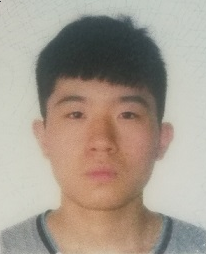
\includegraphics[width=0.88in]{avatar}} & \scshape{焦伟豪(Wewhao Jiao)} & \pbar{Python}{0.7} \\
    & \email{18742052308@163.com} & \pbar{R}{0.6} \\
    & \phone{(+86) 187-4205-2308} & \pbar{\LaTeX}{0.7} \\
    & \weixin{jwh1187917677} & \pbar{MS Office}{0.85} \\
    % & \github[github.com/junjc9]{https://github.com/junjc9} & \pbar{SQL}{0.85}
  \end{tabu}
}

%% Reference
%\newpage
%\bibliographystyle{IEEETran}
%\bibliography{mycite}
\end{document}
